\section{Related Work}
\label{sec:related_work}

Herlant et. al identified that mode switching consumes about 17.4\% of execution time even for able bodied users~\cite{herlant2016assistive}. Thus, they proposed an algorithm to automatically switch the modes in order to minimize the time taken to complete the task. This algorithm was tested on three different levels~\cite{herlant2016assistive}:
\begin{enumerate}
    \item \textbf{Manual}: The user has full control over mode switching; the robot provides no assistance
    \item \textbf{Automatic}: The robot automatically switches the mode whenever it enters a new region based determined by an optimality map. This change happens the first time the robot enters the zone. The user can change the mode as they please.
    \item \textbf{Forced}: The robot automatically switches the mode to the time-optimal mode. However, after every action the user took, the robot would switch back to the time-optimal mode.
\end{enumerate}

\begin{figure}[t!]
    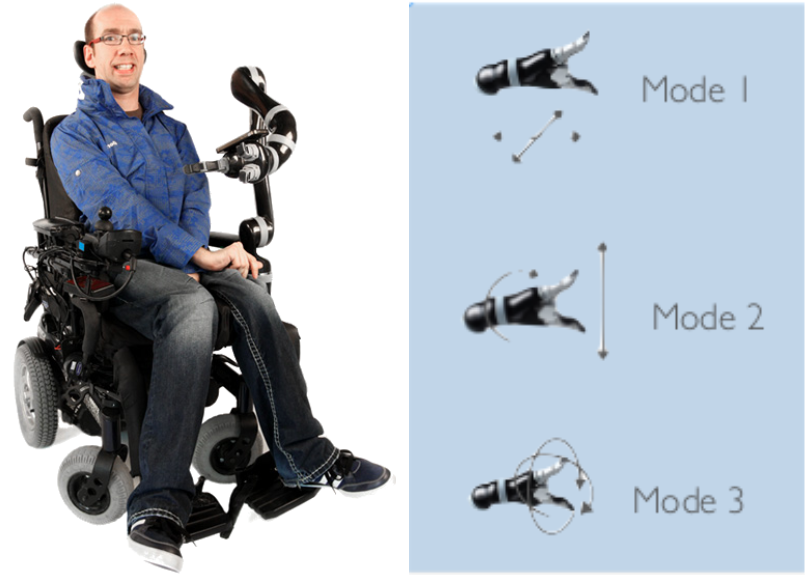
\includegraphics[width=\columnwidth]{figs/kinova}
    \caption{On the left is a figure of a Kinova JACO mounted to a wheelchair~\protect\cite{kinova} that must be controlled by changing between a series of modes~\protect\cite{modes}.}
    \label{fig:kinova}
\end{figure}

Herlant et. al examined the assistance types through task performance and user satisfaction. However, trust is also an essential component in scenarios where a robot and human must work together to reach a common goal~\cite{atkinson2014shared}. Thus, we are interested in exploring how human trust varies as a robot provides different levels guidance through assistive teleoperation. 

In order to test the effectiveness of the assistance the robot provides, we must be able to measure trust. Yagoda et. al grouped trust into three categories: \textit{performance}, \textit{function} and \textit{semantics}~\cite{yagoda2012you}. There are two basis of trust in the performance category that are relevant to our work. The first is \textbf{timely} which is task completion occuring at a favorable time. The second is \textbf{dependability} which is the degree to which behavior is consistent and expected. 